\chapter{Linguaggi visuali}

    Nei precedenti capitoli ho parlato spesso di linguaggi verbali e linguaggi visuali e di quanto la comunicazione visuale può essere più efficiente della comunicazione verbale. In questo capitolo entrerò nel dettaglio senza dilungarmi, andando ad illustrare quali sono le principali differenze tra un linguaggio visuale ed uno verbale, i componenti che lo compongono e in quali casi o contesti un linguaggi visivo è più efficace rispetto ad uno verbale.

    \section{Linguaggio verbale}
        Il linguaggio verbale è un gruppo di elementi, come suoni e parole, che messe insieme formano frasi e infine permettono la comunicazione fra individui. Da questo deriva la comunicazione verbale che è quindi costituita dalle parole usate quando parliamo o scriviamo.

    \section{Componenti}
        Ogni linguaggio è formato da un proprio insieme di componenti. Un linguaggio visuale si distingue principalmente dal linguaggio verbale per i componenti da cui è formato. Il linguaggio visivo si basa su simboli grafici o immagini, elementi che il cervello umano interpreta e trasforma in concetti, linguaggio verbale ed emozioni. Quindi se il linguaggio visuale è costituito da testo e parole per la formazioni di frasi, il linguaggio visivo è formato da simboli e disegni per formare sentenze visive.
        Una componente fondamentale di un linguaggio visuale è il contesto che viene dato ad ogni simbolo appartenente ad una frase visiva.
        \newline
        \begin{figure}[htbp]
            \centering
            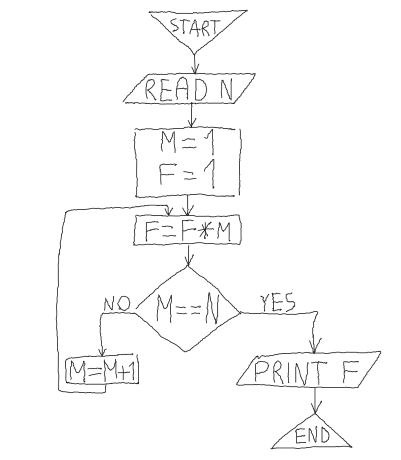
\includegraphics[scale=0.6]{Figure/diagram.PNG}
            \caption{Esempio di sentenza visiva, da~\cite{localcontext_recognition}}
            \label{fig:diagram}
        \end{figure}
        \newline
        Ad esempio, come possiamo notare avvalendoci del disegno in figura~\ref{fig:diagram}, senza un contesto sono semplici simboli connessi fra loro da delle frecce. Invece, dando una definizione ai simboli del diagramma può essere interpretato come un diagramma di flusso o \textit{Flowchart}\footnote{Il diagramma di flusso (o \textit{Flowchart}), in informatica, è una rappresentazione grafica delle operazioni da eseguire per l'esecuzione di un algoritmo.}.

    \section{Vantaggi}
        I vantaggi possono essere molteplici, innanzitutto un linguaggio visuale può essere molto più efficace e di facile comprensione rispetto al linguaggio verbale per via della sua semplicità e naturalità. Non ha lingue o convenzioni in quanto un disegno o un'immagine non dipende da lingue o standard.